%!TEX root = ../main.tex

\section{Tools}
\subsection{Xilinx Suite and Modelsim}
For the designing process, the Microblaze programming, the custom IP cores implementation, and the board programming, the Xilinx tool suite, Xilinx ISE Design Suite 13.1 \cite{xilinx_ise_13_1}, is utilized. For simulating the design, Modelsim is preferred due to its capabilities and direct integration with Xilinx tools.

ISE comprises tools for hardware synthesis in VHDL or Verilog. It provides syntax checking, direct simulation, and hardware synthesis for FPGA programming. This toolset is used for the implementation of the cryptographic algorithms.

An important tool within ISE is the Embedded Development Kit (EDK), which aids in system design, offering an easy instantiation of different processors and a plethora of ready-to-use peripherals. It supports configuration options of several system parameters, such as processor cache size, peripheral addressing schemes, different bus types instantiations, and choice amongst several interfacing options between processors and peripherals. Additionally, custom IP Cores can be easily integrated into the system using EDK. The IPsec system is defined using EDK, the Ethernet, UART, and DDR2 peripherals are added, and the custom cryptographic IP cores AES-128 and HMAC-SHA1-96 are integrated.

Another crucial tool is the Software Development Kit (SDK). It helps manage the system's software, from implementing a simple routine to loading a full-fledged operating system onto processors (e.g., Xilkernel or embedded Linux). It supports programming in C, C++, and assembly. Moreover, it offers ready-to-use software systems such as the lwIP protocol stack and the Xilkernel operating system. From this tool, the software can be downloaded and run in an FPGA system. Software debugging is also performed using SDK. Finally, it includes monitoring of a serial port, allowing us to receive program messages through STDIO (standard input-output). The IPsec code is developed and integrated into the lwIP library using this tool.

Modelsim is a widely used hardware simulator program. It is directly integrated into ISE, which eliminates the need to manually include Xilinx libraries in Modelsim. Furthermore, it provides automation capabilities for simulation, based on the Tcl language, boosting productivity during design 
 debugging and verification. Tcl is used during the CBC-AES-128 verification, in order to automatically simulate and verify the design's correctness against the FIPS test vectors.

\subsection{Wireshark}
Wireshark \cite{wireshark_wiki} is one of the most famous traffic analyzers. Its primary function is to monitor a network interface (e.g., Ethernet, Wi-Fi, etc.) and display the packets moving through it. It is extensively used during the IPsec implementation and testing phase to aid in software debugging.

Wireshark conveniently presents packets, recognizing a vast range of protocols and displaying all fields of each protocol in a structured manner. Additionally, packets can be displayed in their "raw" form, i.e., in binary or hexadecimal representation, a feature that is particularly helpful in the debugging of cryptographic algorithms. For the AH and ESP protocols, it provides automatic integrity checking and decryption if the specific SA is provided. Lastly, it offers traffic filtering with a wide range of options which is useful for displaying only packets of interest and avoiding a noisy display of all packets present in real networks.

\subsection{Scapy}
Scapy \cite{Scapy_documentation} is a tool based on the Python programming language. It provides a command language for creating packets of any layer of the stack. It can also send the crafted packet and receive and report responses to them. With Scapy, both predefined packets such as IP, TCP, UDP, etc., can be created as well as packets from their hexadecimal form (Raw).

Scapy is used for debugging and verification of the system's inbound dataflow. By connecting a PC to the FPGA, we can create and send individually crafted packets targeting specific behaviors of the input code of IPsec.

\subsection{Linux ipsec-tools}
The ipsec-tools is the implementation of IPsec for the Linux operating system. It allows us to define SPs and SAs either manually or using IKE.

ipsec-tools is used in the final phase of the implementation as a reference system for the final verification stage. Specifically, ipsec-tools is installed on a computer which is connected to the FPGA. Then, SPs and SAs are defined manually on both the computer and the FPGA. Theis setup allows for verification of the implementation against a real-world system running IPsec.

One might notice that using Scapy in debugging is redundant since ipsec-tools can replace its functionality. The power of Scapy comes from allowing segmented testing, providing fine-grained access to every packet detail, whereas ipsec-tools would require significant effort in additional development to achieve the same. 

\section{Final System Design and Implementation}
Figure \ref{fig:figure_7.1} depicts the high-level diagram of the complete system. The diagram distinguishes which parts are implemented on the FPGA chip and which are located on the board. Microblaze, its peripherals, and a local memory are situated within the FPGA chip. Microblaze is connected to its peripherals via a PLB bus. All peripherals are memory-mapped. The interfaces of the CBC-AES-128 and HMAC-SHA1-96 peripherals are also presented, detailing their registers.

The FPGA chip, external RAM, the serial port (UART) interface and the Ethernet interface are located on the board.

Received incoming packets are placed in a FIFO by the Ethernet interface. The next available packet in FIFO is moved from the Ethernet interface to the Ethernet Controller when the latter is ready. The Ethernet Controller then notifies the Microblaze via an interrupt. The Microblaze interrupts its operation and executes the lwIP Ethernet code responsible for incoming packets, which stores the new packet in RAM, processes the Ethernet packet, and then passes the execution control to the protocol encapsulating the Ethernet packet. In the case of an IP packet, ip\_input is executed next. In the case of an IPsec packet, the payload of the IP packet is passed to ipsec\_input, which checks the SPD and SADB databases, distinguishes between AH or ESP packets, and executes the appropriate function. When it reaches the point of authentication and/or decryption, the execution control proceeds to the corresponding driver. The driver copies blocks of the payload from RAM to the peripheral, issues the appropriate commands, waits for a response from the peripheral, and finally copies the result back to RAM. Once IPsec processing is completed, the payload of the IPsec packet is passed to the appropriate higher-layer protocol. The process of processing outgoing packets follows the reverse flow, starting from a higher-layer packet and ending in the output FIFO and finally transmission via the Ethernet interface. Lastly, during IPsec execution, debugging messages are generated and sent through the UART interface to a PC.

% fig 7.1
\begin{figure}
\centering
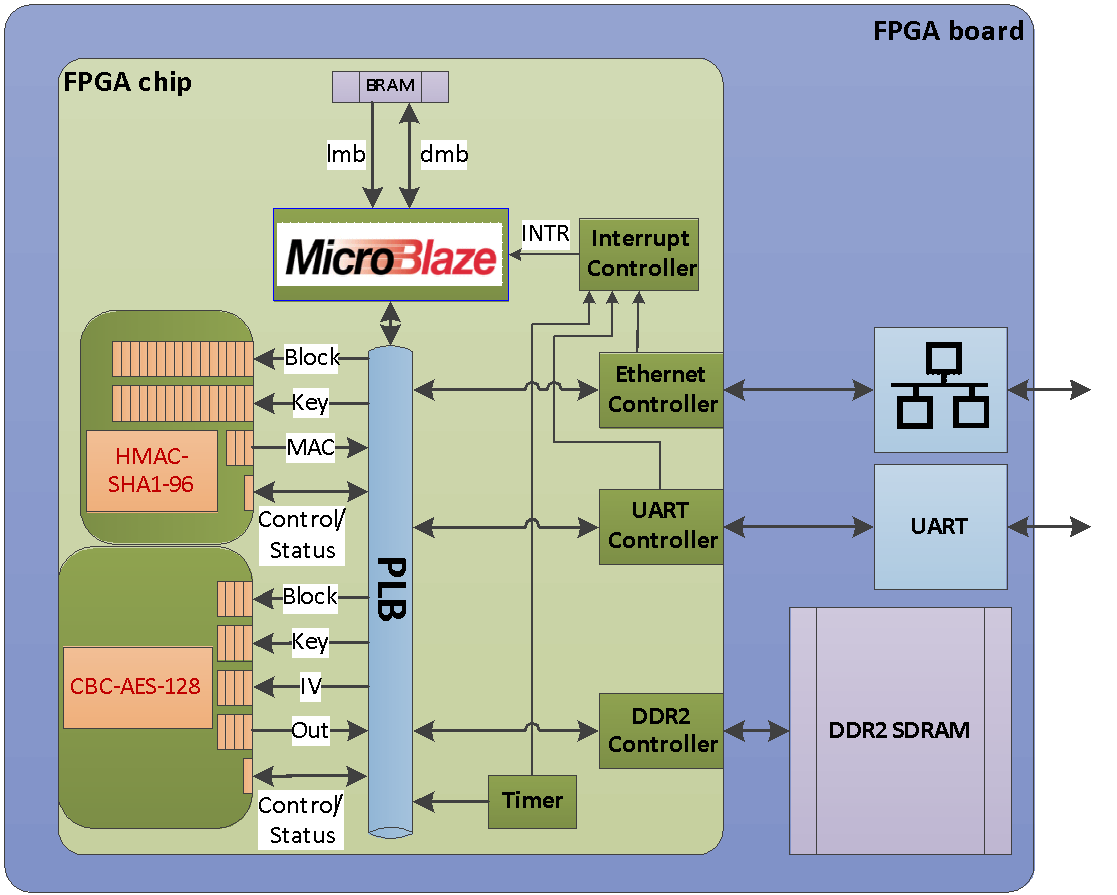
\includegraphics[width= 0.8\textwidth]{figure_7.1}\\
\caption{ Complete system architecture. }
\label{fig:figure_7.1}
\end{figure}

\section{On-Chip Verification}
An ECHO server is implemented for testing the system's operation in a near-real application scenario. The ECHO server accepts requests that carry a message and responds to the requester, echoing back the same message. The server is deployed on the FPGA. The setup is shown in Figure \ref{fig:figure_7.2}. 

A Ruby script served as a client of the ECHO server. It establishes a connection with the server and then sends ECHO requests. The code snippet shown in Listing \ref{lst:echo_client}, serves as an example of a client. It connects to the ECHO server and then sends 1000 randomly sized messages with a payload ranging from 5 to 50 random uppercase characters. If a disparity between the request and response arises, the transmission halts and the fault is reported. Finally, the connection is closed.\\

\noindent
\begin{minipage}{\linewidth}
\begin{lstlisting}[style=mycodestyle, label={lst:echo_client}, caption={ECHO client Ruby implementation}]
require ‘socket’
cl=TCPSocket.new(Server_IP, 7)
for i in 0..1000
 	    random_message = (0..(rand(50)+5).map{ (65+rand(26)).chr }.join
    cl.puts random_message
    if cl.gets != random_message then
        puts “Unexpected Response”
        break
    end
end
cl.close  
\end{lstlisting}
\end{minipage}\\

% fig 7.2
\begin{figure}
\centering
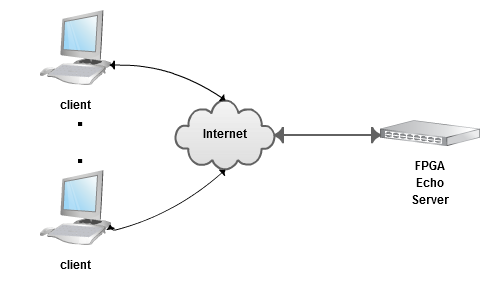
\includegraphics[width= 0.8\textwidth]{figure_7.2}\\
\caption{ ECHO server in Transport Mode }
\label{fig:figure_7.2}
\end{figure}

The preparation of the setup includes configuring the policies in the SPD and the SAs in the SADB \cite{setkey_manpage} of both systems and setting up Wireshark for collecting the relevant packets. The system is tested for both protocols (AH and ESP) using a large number of packets. As an example, the packets of one request-response scenario are presented in Figures \ref{fig:figure_7.3}, \ref{fig:figure_7.4}, \ref{fig:figure_7.5},  \ref{fig:figure_7.6}, \ref{fig:figure_7.7} and \ref{fig:figure_7.8}.

\subsubsection*{ESP with CBC-AES-128 and HMAC-SHA1-96 in Transport Mode}

Initially, an ECHO Request with the message "abc" is sent from the client to the server located on the FPGA. The encrypted ESP packet is presented in Figure \ref{fig:figure_7.3}. The colored fields are, in order of appearance:
\begin{outline}
    \1 Ethernet Header
    \1 IP Header
    \1 SPI
    \1 Sequence Number
    \1 IV
    \1 Payload
    \1 ICV
\end{outline}

Figure \ref{fig:figure_7.4} depicts the decrypted payload. The first field is the TCP packet, which, as indicated in the ASCII view, contains the "abc" message. The padding, pad length, and next header follow as part of the second field. The last field is the ICV.

% fig wireshark 1
\begin{figure}[H]
\centering
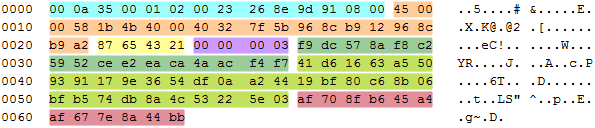
\includegraphics[width= 0.8\textwidth]{figure_7.3}\\
\caption{ Transmitted packet of ECHO request in ESP Transport Mode  }
\label{fig:figure_7.3}
\end{figure}

Next, the ECHO server on the FPGA responds. The response is shown in Figure \ref{fig:figure_7.5}.

% fig wireshark 2
\begin{figure}[H]
\centering
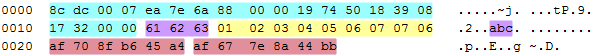
\includegraphics[width= 0.8\textwidth]{figure_7.4}\\
\caption{ Decrypted payload of the ECHO request in ESP Transport Mode }
\label{fig:figure_7.4}
\end{figure}

We observe the presence of the SPI, Sequence Number, IV fields, the encrypted payload, and the ICV. The decrypted packet of the response is shown in Figure \ref{fig:figure_7.6}.

% fig wireshark 3
\begin{figure}[H]
\centering
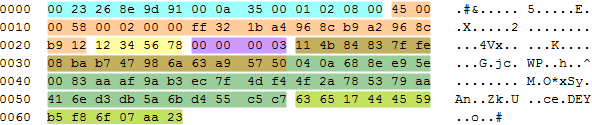
\includegraphics[width= 0.8\textwidth]{figure_7.5}\\
\caption{ ECHO server response in ESP Transport Mode }
\label{fig:figure_7.5}
\end{figure}

We observe that the original message of the request, 'abc', exists in the decrypted payload.

\subsubsection*{AH with HMAC-SHA1-96 in Transport Mode}
Initially, an ECHO Request with the message "abc" is sent from the client to the server located on the FPGA. The AH packet is presented in Figure \ref{fig:figure_7.7}. The colored fields are in the order of appearance:

\begin{outline}
    \1 Ethernet Header
    \1 IP Header
    \1 Next Header
    \1 AH Length
    \1 Reserved
    \1 SPI
    \1 Sequence Number
    \1 ICV
    \1 TCP Payload
    \1 ECHO Payload    
\end{outline}


% fig wireshark 4
\begin{figure}[H]
\centering
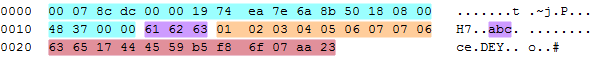
\includegraphics[width= 0.8\textwidth]{figure_7.6}\\
\caption{ Decrypted payload of ECHO server response in ESP Transport Mode }
\label{fig:figure_7.6}
\end{figure}

% fig wireshark 5
\begin{figure}[H]
\centering
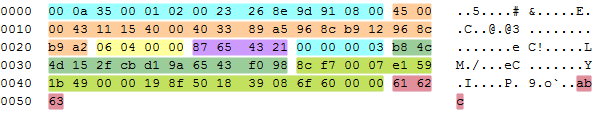
\includegraphics[width= 0.8\textwidth]{figure_7.7}\\
\caption{ Transmitted packet of ECHO request in AH Transport Mode }
\label{fig:figure_7.7}
\end{figure}

\begin{figure}[H]
\centering
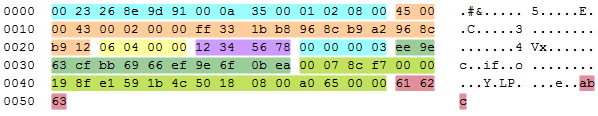
\includegraphics[width= 0.8\textwidth]{figure_7.8}\\
\caption{ ECHO server response in AH Transport Mode}
\label{fig:figure_7.8}
\end{figure}

\noindent
The FPGA's response is shown in Figure \ref{fig:figure_7.8}.
We observe the presence of the fields in the AH header, as well as the correct content in the ECHO payload.

\section{Evaluation}
Data collection of performance metrics is performed. The purpose of these measurements is to estimate the system's performance and calculate the efficiency gains that the hardware cryptographic algorithms offer compared to a software-only implementation. The metric measured is the number of clock cycles required for processing a packet from the moment it enters the processing path we want to measure. An on-chip timer is used for counting clock cycles. When IPsec processing begins, the timer is initialized and activated. Upon activation, the timer increments its counter value by one at each clock cycle. To measure the processing time of a particular path, we store the timer value at the beginning and end. Subtracting these two quantities yields the number of clock cycles that the specific execution path took.

For comparison with a software-only implementation, the same system is modified using software cryptographic algorithms. The algorithms are implemented based on the OpenSSL package, with minor modifications for porting the code to our system. This decision is made because the implementation of the algorithms in OpenSSL is highly optimized and thus it provides a competitive comparison.

The measurements were conducted using the ESP protocol since it uses both cryptographic algorithms. The measurements are divided into two parts, one for the processing of incoming packets and one for the processing of outgoing ones. Additionally, various payload sizes are used to provide a complete performance picture, as there are parts of the system whose processing time is dependent on the packet size. The paths measured include the total processing of IPsec, the ESP processing, and both of the cryptographic algorithms. It should be noted that the measurement of IPsec includes ESP processing, and ESP includes the cryptographic algorithms execution. The measurements are presented in Table \ref{table:7.1} for inbound traffic and in Table \ref{table:7.2} for outbound traffic. The quantities are expressed in the number of clock cycles.

The tables include a row labeled 'Speedup,' indicating how many times faster the hardware implementation of the measured part is compared to the software implementation. This calculation is the division of the number of clock cycles of the software implementation by those of the hardware implementation. Two additional columns are added for the processing time of only the ESP header (i.e., without the cryptographic algorithms) and for the processing time of the IPsec without ESP processing (i.e., including the IPsec header processing and searches in the SPD and SADB).

% table 7.1
% Please add the following required packages to your document preamble:
% \usepackage{multirow}
% \usepackage[table,xcdraw]{xcolor}
% Beamer presentation requires \usepackage{colortbl} instead of \usepackage[table,xcdraw]{xcolor}
\begin{table}[]
\centering
\begin{tabular}{llllllll}
\toprule
% \multicolumn{8}{|c|}{\textbf{Inbound packet processing}} \\
% \hline
\textbf{\begin{tabular}[|c|]{@{}l@{}}Payload\\ size\\ (bytes)\end{tabular}} &    &     &     &   &   & \textbf{\begin{tabular}[c]{@{}l@{}}ESP \\ Header\\  Processing\end{tabular}} & \textbf{\begin{tabular}[c]{@{}l@{}}IPsec \\ Header\\  Processing\end{tabular}} \\
      & \multirow{-3}{*}{\textbf{HW/SW}} & \multirow{-3}{*}{\textbf{AES}} & \multirow{-3}{*}{\textbf{HMAC}} & \multirow{-3}{*}{\textbf{ESP}}  & \multirow{-3}{*}{\textbf{IPsec}}   &  & \\
      \hline
      & SW	 & 772693	 & 279229	 & 1054804	 & 1057353 & 2882       & 2549 \\
      & HW    & 17625     & 49741     & 70174   & 72724   & 2808       & 2550 \\
\multirow{-3}{*}{\textbf{3}}     & {\color[HTML]{00B050} \textbf{Speedup}}   & {\color[HTML]{00B050} \textbf{43.84}}   & {\color[HTML]{00B050} \textbf{5.61}} & {\color[HTML]{00B050} \textbf{15.03}} & {\color[HTML]{00B050} \textbf{14.54}} & -       & - \\
\midrule
      & SW    & 771658    & 279396    & 1053938    & 1056474    & 2884       & 2536 \\
      & HW    & 17598     & 49697     & 70104   & 72640   & 2809       & 2536 \\
\multirow{-3}{*}{10}    & {\color[HTML]{00B050} \textbf{Speedup}}   & {\color[HTML]{00B050} \textbf{43.85}}   & {\color[HTML]{00B050} \textbf{5.62}} & {\color[HTML]{00B050} \textbf{15.03}} & {\color[HTML]{00B050} \textbf{14.54}} & -       & - \\
\midrule
      & SW    & 3062302   & 316804    & 3381984    & 3384517    & 2878       & 2533 \\
      & HW    & 59600     & 63569     & 125973  & 128503  & 2804       & 2530 \\
\multirow{-3}{*}{100}      & {\color[HTML]{00B050} \textbf{Speedup}}   & {\color[HTML]{00B050} \textbf{51.38}}   & {\color[HTML]{00B050} \textbf{4.98}} & {\color[HTML]{00B050} \textbf{26.85}} & {\color[HTML]{00B050} \textbf{26.34}} & -       & - \\
\midrule
      & SW    & 12619006     & 589613    & 13211500   & 13214036   & 2881       & 2536 \\
      & HW    & 234658    & 132484    & 369958  & 372492  & 2816       & 2534 \\
\multirow{-3}{*}{500}      & {\color[HTML]{00B050} \textbf{Speedup}}   & {\color[HTML]{00B050} \textbf{53.78}}   & {\color[HTML]{00B050} \textbf{4.45}} & {\color[HTML]{00B050} \textbf{35.71}} & {\color[HTML]{00B050} \textbf{35.47}} & -       & - \\
\midrule
      & SW    & 24467280     & 947749    & 25417904   & 25420434   & 2875       & 2530 \\
      & HW    & 451749    & 226794    & 681356  & 683890  & 2813       & 2534 \\
\multirow{-3}{*}{1000}     & {\color[HTML]{00B050} \textbf{Speedup}}   & {\color[HTML]{00B050} \textbf{54.16}}   & {\color[HTML]{00B050} \textbf{4.18}} & {\color[HTML]{00B050} \textbf{37.3}}  & {\color[HTML]{00B050} \textbf{37.17}} & -       & -     \\
\bottomrule
\end{tabular}
\caption{Inbound packet processing time (in number of clock cycles)}
\label{table:7.1}
\end{table}\\


% table 7.2
\begin{table}[]
\centering
\begin{tabular}{llllllll}
\toprule
% \multicolumn{8}{|c|}{\textbf{Outbound packet processing}} \\
% \hline
\textbf{\begin{tabular}[|c|]{@{}l@{}}Payload\\ size\\ (bytes)\end{tabular}} & & & & & & \textbf{\begin{tabular}[|c|]{@{}l@{}}ESP\\ Header\\  Processing\end{tabular}} & \textbf{\begin{tabular}[c]{@{}l@{}}IPsec\\ Header\\  Processing\end{tabular}} \\
      & \multirow{-3}{*}{\textbf{HW/SW}} & \multirow{-3}{*}{\textbf{AES}} & \multirow{-3}{*}{\textbf{HMAC}} & \multirow{-3}{*}{\textbf{ESP}}  & \multirow{-3}{*}{\textbf{IPsec}}  & & \\
      \hline
      & SW	 & 543519	 & 269921	 & 867940	 & 871315 & 54500      & 3375 \\
      & HW    & 17600     & 44479     & 117063  & 120437  & 54984      & 3374 \\
\multirow{-3}{*}{\textbf{3}}     & {\color[HTML]{00B050} \textbf{Speedup}}   & {\color[HTML]{00B050} \textbf{30.88}}   & {\color[HTML]{00B050} \textbf{6.07}} & {\color[HTML]{00B050} \textbf{7.41}}  & {\color[HTML]{00B050} \textbf{7.23}}  & -       & - \\
\midrule
      & SW    & 813759    & 267691    & 1137568    & 1140943    & 56118      & 3375 \\
      & HW    & 17587     & 44484     & 116538  & 119899  & 54467      & 3361 \\
\multirow{-3}{*}{10}    & {\color[HTML]{00B050} \textbf{Speedup}}   & {\color[HTML]{00B050} \textbf{46.27}}   & {\color[HTML]{00B050} \textbf{6.02}} & {\color[HTML]{00B050} \textbf{9.76}}  & {\color[HTML]{00B050} \textbf{9.52}}  & -       & - \\
\midrule
      & SW    & 2165365   & 312021    & 2534846    & 2538223    & 57460      & 3377 \\
      & HW    & 59585     & 58280     & 175613  & 178991  & 57748      & 3378 \\
\multirow{-3}{*}{100}      & {\color[HTML]{00B050} \textbf{Speedup}}   & {\color[HTML]{00B050} \textbf{36.34}}   & {\color[HTML]{00B050} \textbf{5.35}} & {\color[HTML]{00B050} \textbf{14.43}} & {\color[HTML]{00B050} \textbf{14.18}} & -       & - \\
\midrule
      & SW    & 8911300   & 582429    & 9560500    & 9563879    & 66771      & 3379 \\
      & HW    & 234655    & 127235    & 429579  & 432952  & 67689      & 3373 \\
\multirow{-3}{*}{500}      & {\color[HTML]{00B050} \textbf{Speedup}}   & {\color[HTML]{00B050} \textbf{37.98}}   & {\color[HTML]{00B050} \textbf{4.58}} & {\color[HTML]{00B050} \textbf{22.26}} & {\color[HTML]{00B050} \textbf{22.09}} & -       & - \\
\midrule
      & SW    & 17275837     & 943116    & 18296571   & 18299937   & 77618      & 3366 \\
      & HW    & 451705    & 221543    & 751779  & 755145  & 78531      & 3366 \\
\multirow{-3}{*}{1000}     & {\color[HTML]{00B050} \textbf{Speedup}}   & {\color[HTML]{00B050} \textbf{38.25}}   & {\color[HTML]{00B050} \textbf{4.26}} & {\color[HTML]{00B050} \textbf{24.34}} & {\color[HTML]{00B050} \textbf{24.23}} & -       & -     \\
\bottomrule
\end{tabular}
\caption{Outbound packet processing time (in number of clock cycles)}
\label{table:7.2}
\end{table}


First, we observe that the system benefits from the implementation of cryptographic algorithms in hardware for both inbound and outbound traffic, for every examined packet size. This is evident from the positive values in the Speedup row of the IPsec column. Furthermore, we notice that the Speedup of IPsec increases as the packet size grows. Further analysis of the measurements reveals that the dominant factor in the system's speedup is CBC-AES-128. HMAC-SHA1-96 contributes to the speedup but to a much lesser extent. Additionally, the trend of the speedup to increase as packets grow larger is also attributed to CBC-AES-128. Conversely, HMAC-SHA1-96 appears to decrease in speedup as packet size increases, but this trend is less pronounced than that of CBC-AES-128 and does not have a significant impact on system performance. Finally, the processing of headers and searches in SPD and SADB remains consistent, as expected since their implementation remains unchanged. Any slight deviation observed between them is due to non-deterministic factors such as the search time in databases. Lastly, when comparing the measurements between inbound and outbound traffic, a difference in the processing of the ESP header is identified. This difference is attributed to the fact that during header creation in outbound traffic, a random IV and padding are generated, processes that do not exist in inbound processing, which leads to increased memory copies compared to inbound processing.

From the above measurements, the system's throughput can be easily calculated using Equation \ref{eq:throughput}, where $\#bits$ represents the number of bits processed in time.

\begin{equation}\label{eq:throughput}
    Throughput = \frac{\#bits}{time }
\end{equation}

Knowing the number of clock cycles and the operating frequency of the system, we can determine how much time is required to process a packet using Equation \ref{eq:time}, where $f = 100MHz$ is the operating frequency and $\#clk$ is the number of clock cycles. 


\begin{equation}\label{eq:time}
    time = \frac{\#clk}{f}
\end{equation}


\noindent
Combining Equations \ref{eq:throughput} and \ref{eq:time} we get the final throughput formula in Equation \ref{eq:throughput_final}.

\begin{equation}\label{eq:throughput_final}
    Throughput=\frac{\#bits*100*10^6}{\#clk}
\end{equation}

Using Equation \ref{eq:throughput_final}, we can calculate the throughput of our system across all packet sizes. Here, it should be noted that $\#bits$ represent the size of the packet payload, excluding the header, padding, IV, and trailer. Table \ref{table:7.3} presents the throughput calculations for the aforementioned payload sizes for inbound and outbound traffic. The Graph \ref{fig:throughput_graph} summarizes the table. We observe significant improvement from the use of hardware cryptographic algorithms, especially for medium to large packets. Furthermore, we notice that the throughput trend is increasing as packet size increases.


% table 7.3
\begin{table}[]
\centering
% \begin{tabularx}{0.7\textwidth}{|l|ll|ll|}
\begin{tabularx}{0.6\textwidth} { 
  | >{\raggedleft\arraybackslash}X 
  | >{\raggedright\arraybackslash}X >{\raggedright\arraybackslash}X
  | >{\raggedright\arraybackslash}X >{\raggedright\arraybackslash}X | }
% \multicolumn{5}{l}{\textbf{Throughput (KB/s)}} \\
\hline
\multirow{2}{*}{\textbf{\#bits}} & \multicolumn{2}{c|}{\textbf{Outbound}} & \multicolumn{2}{c|}{\textbf{Inbound}} \\
   & \multicolumn{1}{c}{\textbf{HW}}   & \multicolumn{1}{c|}{\textbf{SW}}  & \multicolumn{1}{c}{\textbf{HW}}   & \multicolumn{1}{c|}{\textbf{SW}} \\
\hline
3  & 19.93   & 2.75   & 33   & 2.27 \\
10    & 66.72   & 7.01   & 110.13  & 7.57 \\
100   & 446.95  & 31.52  & 622.55  & 23.64 \\
500   & 923.89  & 41.82  & 1073.85 & 30.27 \\
1000  & 1059.4  & 442.62 & 1169.78 & 31.47 \\   
\hline
\end{tabularx}
\caption{Throughput (KB/s)}
\label{table:7.3}
\end{table}\\


\begin{figure}
    \centering
    
\begin{tikzpicture}
\begin{axis}[
    % width=10cm,
   % height=4cm,
   scale only axis,
   xmin=0, xmax=1100,
   xtick={10,100, 1000},
   xticklabels={10,100, 1000},
   xmajorgrids,
   ymin=0, ymax=1200,
   ylabel={$Througput[KB/s]$},
   ymajorgrids,
   % title={Throughput comparison},
   axis lines*=left,
%  line width=1.0pt,
%  mark size=2.0pt,
   legend cell align={left},
   legend style ={ at={(1.03,1)}, 
        anchor=north west, draw=black, 
        fill=white,align=left,
        row sep=2pt},
    cycle list name=black white,
    smooth
]

    \addplot[line width=1pt,mark size=4pt, mark=*] coordinates{
(3, 19.93)
(10, 66.72)
(100, 446.95)
(500, 923.89)
(1000, 1059.4)
    };
    \addlegendentry{Software throughput \\for outbound flow };

   \addplot[[line width=1pt,mark size=4pt, mark=square] coordinates{
(3, 33)
(10, 110.13)
(100, 622.55)
(500, 1073.85)
(1000, 1169.78)
    };
   \addlegendentry{Software throughput \\for inbound flow};

   \addplot[[line width=1pt,mark size=4pt, mark=triangle] coordinates{
(3, 2.75)
(10, 7.01)
(100, 31.52)
(500, 41.82)
(1000, 442.62)
    };
    \addlegendentry{Hardware throughput \\for outbound flow};
    
   \addplot[[line width=1pt,mark size=4pt, mark=diamond] coordinates{
(3, 2.27)
(10, 7.57)
(100, 23.64)
(500, 30.27)
(1000, 31.47)
    };
    \addlegendentry{Hardware throughput \\for inbound flow}

   \end{axis}
\end{tikzpicture}%
    \caption{Throughput comparisons across SW/HW and inbound/outbound flows}
    \label{fig:throughput_graph}
\end{figure}

Furthermore, the area utilization of the implemented system and the peripherals are measured. Table \ref{table:7.4} summarizes the results. The percentages refer to the peripheral area relative to the total system area.


% table 7.4
\begin{table}[]
\centering
\begin{tabular}{l|cc|cc|c|}
\hline
% \multicolumn{6}{l}{\textbf{Area}} \\
\multirow{2}{*}{\textbf{Metrics}} &
\multirow{2}{*}{\textbf{CBC-AES-128}} & 
\multirow{2}{*}{\textbf{\%}} & 
\multirow{2}{*}{\textbf{HMAC-SHA1-96}} & 
\multirow{2}{*}{\textbf{\%}} & 
\multirow{2}{*}{\textbf{System Total}} \\
    &   &   &    &   & \\
\hline
Registers    & 1808    & 15.41   & 1535     & 13.08   & 11732 \\
LUTs   & 3018    & 24.12   & 1318     & 10.53   & 12511 \\
Slices    & 1108    & 18   & 456   & 7.41    & 6154    \\
\hline
\end{tabular}
\caption{Area utilization}
\label{table:7.4}
\end{table}
